\question (中山大学,2004年)采用双亲表示法表示树,则具有n个结点的树至少需要(
)个指向双亲的指针
\par\twoch{n}{n+1}{\textcolor{red}{n-1}}{2n}
\begin{solution}除了根结点,其他结点都指向双亲,因此有n-1个指向双亲的指针。
\end{solution}
\question 在一棵度数为4的树T中,若有20个度为4的结点,10个度为3的结点,1个度为2的结点,10个度为1的结点,则树T的叶结点个数是(
)
\par\twoch{41}{\textcolor{red}{82}}{113}{122}
\begin{solution}设树的总结点数为n,由于树T的度为4,故树T只能有度为0、1、2、3、4的结点。设ni为度为i的结点数。n=n0+n1+n2+n3+n4(其中n0即为叶结点的个数)。在一棵树中,度之和=结点数-1=n-1。又度之和=1×n1+2×n2+3×n3+4×n4=1×10+2×1+3×10+4×20=122。即n-1=122,得到n=123。n0=n-n1-n2-n3-n4=123-10-1-10-20=82。
【总结】 树的度之和=分支数=结点数减1。
\end{solution}
\question 求下面带权图的最小(代价)生成树时,可能是克鲁斯卡(kruskal)算法第二次选中但
不是普里姆(Prim)算法(从V4 开始)第2 次选中的边是

~
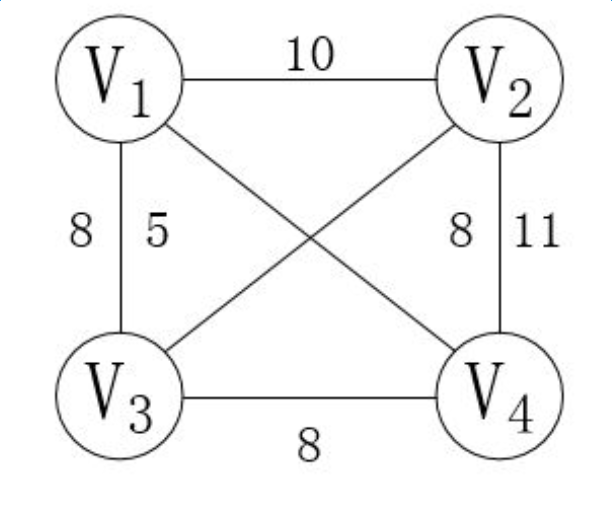
\includegraphics[width=1.04167in,height=1.04167in]{computerassets/96705ACDEE416EAA788ED33A0F97461B.png}
\par\fourch{\textcolor{red}{(V1,V3)}}{(V1,V4)}{(V2,V3)}{(V3,V4)}
\begin{solution}最小生成树算法的Prim 算法和Kruskal 算法。
\end{solution}
\question (上海交通大学,2005年)树中所有节点的度等于所有节点数加( )
\par\twoch{0}{1}{\textcolor{red}{-1}}{2}
\begin{solution}若树中只有根节点,则度为0,节点数为1;每添加一个节点,则节点数加1,所有节点的度也加1;故树中所有节点的度等于所有节点数减1
\end{solution}
